\documentclass[tikz,border=10pt]{standalone}
\usepackage{tikz}
\usepackage{pgfplots}
\pgfplotsset{compat = 1.18, width = 10cm}
\usetikzlibrary{calc, arrows, positioning, shapes.geometric}
\usepackage{tikz-dimline}
\usepackage{tkz-euclide}
\usetikzlibrary{backgrounds}
\usetikzlibrary{patterns}
\usepgfplotslibrary{fillbetween, groupplots}
\input{Core Tikz Library/colours}

\begin{document}

% Q1
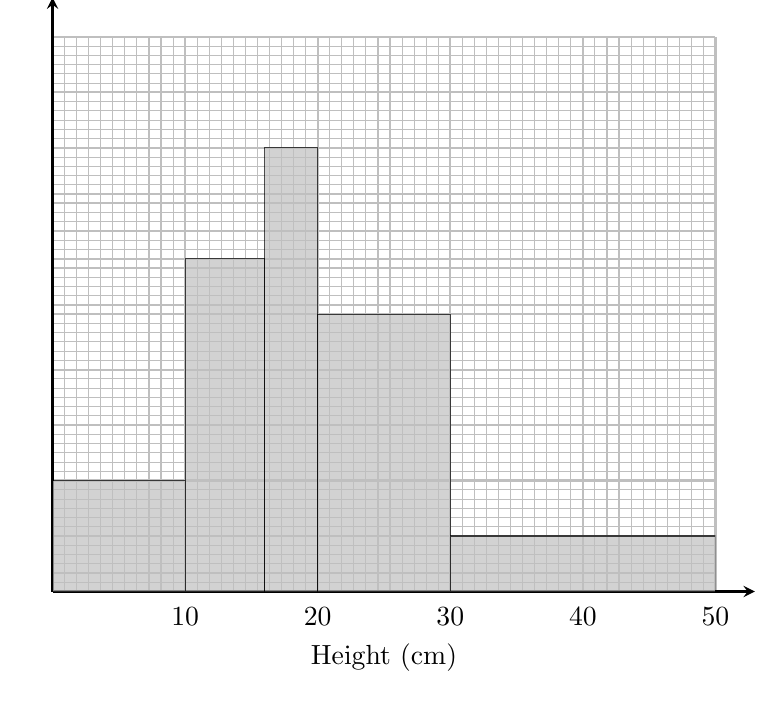
\begin{tikzpicture}
 \begin{axis}[width=10cm,
     axis lines=center,
     axis line style = {line width = 1.5pt, shorten >=-5mm},
     xmin=0,xmax=50,
     ymin=0,ymax=10,
     grid=major,
     yminorgrids,
     xminorgrids,
     ylabel near ticks,
     xlabel near ticks,
     major grid style={thick},
     tick style={thick},
     axis line style={thick},
     xlabel= Height (cm),
     ylabel=,
     xtick={0,10,...,50},
     ytick={0,1,2,...,10},
     yticklabels={},
     minor y tick num=5,
     minor x tick num=10,
     ytick style={draw=none},
     xtick style={draw=none},
     ]
    \addplot[ybar interval,fill=gray!50,draw=black, opacity = 0.7]coordinates{(0,2)(10,0)};
    \addplot[ybar interval,fill=gray!50,draw=black, opacity = 0.7]coordinates{(10,6)(16,2)};
    \addplot[ybar interval,fill=gray!50,draw=black, opacity = 0.7]coordinates{(16,8)(20,0)};
    \addplot[ybar interval,fill=gray!50,draw=black, opacity = 0.7]coordinates{(20,5)(30,0)};
    \addplot[ybar interval,fill=gray!50,draw=black, opacity = 0.7]coordinates{(30,1)(50,0)};
  \end{axis}
 \end{tikzpicture}

 % Q2
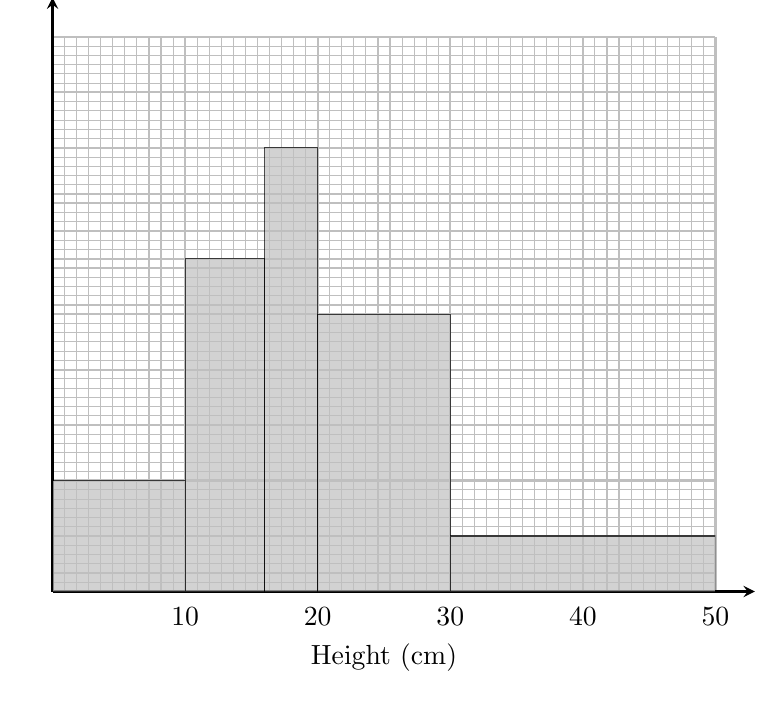
\begin{tikzpicture}
 \begin{axis}[width=10cm,
     axis lines=center,
     axis line style = {line width = 1.5pt, shorten >=-5mm},
     xmin=0,xmax=50,
     ymin=0,ymax=10,
     grid=major,
     yminorgrids,
     xminorgrids,
     ylabel near ticks,
     xlabel near ticks,
     major grid style={thick},
     tick style={thick},
     axis line style={thick},
     xlabel= Height (cm),
     ylabel=,
     xtick={0,10,...,50},
     ytick={0,1,2,...,10},
     yticklabels={},
     minor y tick num=5,
     minor x tick num=10,
     ytick style={draw=none},
     xtick style={draw=none},
     ]
    \addplot[ybar interval,fill=gray!50,draw=black, opacity = 0.7]coordinates{(0,2)(10,0)};
    \addplot[ybar interval,fill=gray!50,draw=black, opacity = 0.7]coordinates{(10,6)(16,2)};
    \addplot[ybar interval,fill=gray!50,draw=black, opacity = 0.7]coordinates{(16,8)(20,0)};
    \addplot[ybar interval,fill=gray!50,draw=black, opacity = 0.7]coordinates{(20,5)(30,0)};
    \addplot[ybar interval,fill=gray!50,draw=black, opacity = 0.7]coordinates{(30,1)(50,0)};
  \end{axis}
 \end{tikzpicture}

\end{document}